\subsection{Construção de Tabelas-Verdade}

\begin{frame}[t]
\vskip 2.5cm
\begin{center}
{\Huge Construção de\\Tabelas-Verdade}
\end{center}
\end{frame}

\begin{frame}[t]{Construção de Tabelas-Verdade} % Título do Frame
	\begin{itemize}
	  \item Número de Linhas = $2^N$, onde N = número de proposições
	  \item Dois Métodos:
	  \begin{enumerate}
	  \item uma coluna por operador 
             \item uma coluna por símbolo
	  \end{enumerate}
	\end{itemize}
\end{frame}

\begin{frame}[t]{Construção de Tabelas-Verdade} % Título do Frame
	Método \#1 - Uma coluna por operador.
	
	\begin{center}
	Exemplo: $\sim (p \wedge \sim q)$
	
	\vskip 0.8cm
		
	\begin{tabular}{|c|c|}
	\hline
	$\mathbf{p}$ & $\mathbf{q}$ \\
	\hline
	V & V \\
	\hline
	V & F \\
	\hline
	F & V \\
	\hline
	F & F \\
	\hline
	\end{tabular}
	\end{center}
\end{frame}

\begin{frame}[t]{Construção de Tabelas-Verdade} % Título do Frame
	Método \#1 - Uma coluna por operador.
	
	\begin{center}
	Exemplo: $\sim (p \wedge \sim q)$
	
	\vskip 0.8cm
		
	\begin{tabular}{|c|c|c|}
	\hline
	$\mathbf{p}$ & $\mathbf{q}$ & $\mathbf{\sim q}$\\
	\hline
	V & V & F\\
	\hline
	V & F & V \\
	\hline
	F & V & F \\
	\hline
	F & F & V \\
	\hline
	\end{tabular}
	\end{center}
\end{frame}

\begin{frame}[t]{Construção de Tabelas-Verdade} % Título do Frame
	Método \#1 - Uma coluna por operador.
	
	\begin{center}
	Exemplo: $\sim (p \wedge \sim q)$
	
	\vskip 0.8cm
		
	\begin{tabular}{|c|c|c|c|}
	\hline
	$\mathbf{p}$ & $\mathbf{q}$ & $\mathbf{\sim q}$ & $\mathbf{p \wedge \sim q}$ \\
	\hline
	V & V & F & F \\
	\hline
	V & F & V & V \\
	\hline
	F & V & F & F \\
	\hline
	F & F & V & F \\
	\hline
	\end{tabular}
	\end{center}
\end{frame}

\begin{frame}[t]{Construção de Tabelas-Verdade} % Título do Frame
	Método \#1 - Uma coluna por operador.
	
	\begin{center}
	Exemplo: $\sim (p \wedge \sim q)$
	
	\vskip 0.8cm
		
	\begin{tabular}{|c|c|c|c|c|}
	\hline
	$\mathbf{p}$ & $\mathbf{q}$ & $\mathbf{\sim q}$ & $\mathbf{p \wedge \sim q}$ & $\mathbf{\sim(p \wedge \sim q)}$ \\
	\hline
	V & V & F & F & V \\
	\hline
	V & F & V & V & F \\
	\hline
	F & V & F & F & V \\
	\hline
	F & F & V & F & V \\
	\hline
	\end{tabular}
	\end{center}
\end{frame}

\begin{frame}[t]{Construção de Tabelas-Verdade} % Título do Frame
	Método \#2 - Uma coluna por símbolo.
	
	\begin{center}
	Exemplo: $\sim (p \wedge \sim q)$
	
	\vskip 0.8cm
		
	\begin{tabular}{|c|c|c|c|c|}
	\hline
	& {\tiny 1} & & & {\tiny 1} \\
	\hline
	\hline
	$\mathbf{\sim}$ & $\mathbf{p}$ & $\mathbf{\wedge}$ & $\mathbf{\sim}$ & $\mathbf{q}$ \\
	\hline
	  & V &   &   & V \\
	\hline
	  & V &   &   & F \\
	\hline
	  & F &   &   & V \\
	\hline
	  & F &   &   & F \\
	\hline
	\end{tabular}
	\end{center}
\end{frame}

\begin{frame}[t]{Construção de Tabelas-Verdade} % Título do Frame
	Método \#2 - Uma coluna por símbolo.
	
	\begin{center}
	Exemplo: $\sim (p \wedge \sim q)$
	
	\vskip 0.8cm
		
	\begin{tabular}{|c|c|c|c|c|}
	\hline
	& {\tiny 1} & & {\tiny 2} & {\tiny 1} \\
	\hline
	\hline
	$\mathbf{\sim}$ & $\mathbf{p}$ & $\mathbf{\wedge}$ & $\mathbf{\sim}$ & $\mathbf{q}$ \\
	\hline
	  & V &   & F & V \\
	\hline
	  & V &   & V & F \\
	\hline
	  & F &   & F & V \\
	\hline
	  & F &   & V & F \\
	\hline
	\end{tabular}
	\end{center}
\end{frame}

\begin{frame}[t]{Construção de Tabelas-Verdade} % Título do Frame
	Método \#2 - Uma coluna por símbolo.
	
	\begin{center}
	Exemplo: $\sim (p \wedge \sim q)$
	
	\vskip 0.8cm
		
	\begin{tabular}{|c|c|c|c|c|}
	\hline
	& {\tiny 1} & {\tiny 3} & {\tiny 2} & {\tiny 1} \\
	\hline
	\hline
	$\mathbf{\sim}$ & $\mathbf{p}$ & $\mathbf{\wedge}$ & $\mathbf{\sim}$ & $\mathbf{q}$ \\
	\hline
	  & V & F & F & V \\
	\hline
	  & V & V & V & F \\
	\hline
	  & F & F & F & V \\
	\hline
	  & F & F & V & F \\
	\hline
	\end{tabular}
	\end{center}
\end{frame}

\begin{frame}[t]{Construção de Tabelas-Verdade} % Título do Frame
	Método \#2 - Uma coluna por símbolo.
	
	\begin{center}
	Exemplo: $\sim (p \wedge \sim q)$
	
	\vskip 0.8cm
		
	\begin{tabular}{|c|c|c|c|c|}
	\hline
	{\tiny 4} & {\tiny 1} & {\tiny 3} & {\tiny 2} & {\tiny 1} \\
	\hline
	\hline
	$\mathbf{\sim}$ & $\mathbf{p}$ & $\mathbf{\wedge}$ & $\mathbf{\sim}$ & $\mathbf{q}$ \\
	\hline
	V & V & F & F & V \\
	\hline
	F & V & V & V & F \\
	\hline
	V & F & F & F & V \\
	\hline
	V & F & F & V & F \\
	\hline
	\end{tabular}
	\end{center}
\end{frame}

\begin{frame}[t]{Construção de Tabelas-Verdade} % Título do Frame
	Concluindo:
	
	\begin{center}Exemplo: $\sim (p \wedge \sim q)$\end{center}

	$$P_{pq}(VV, VF, FV, FF) = (V, F, V, V)$$

	\begin{center}ou\end{center}

	$$P_{pq}(00, 01, 10, 11) = (1, 1, 0, 1)$$
\end{frame}

\begin{frame}[t]{Construção de Tabelas-Verdade - Exercícios} % Título do Frame
	\begin{enumerate}
	\item $\sim (p \wedge q) \vee\sim (q \leftrightarrow p)$
	\item $p \vee\sim r \rightarrow q \wedge\sim r$
	\item $(p \rightarrow q) \wedge (q \rightarrow r) \rightarrow (p \rightarrow r)$
	\end{enumerate}
\end{frame}

\begin{frame}[t]{Construção de Tabelas-Verdade - Exercícios} % Título do Frame
	\begin{enumerate}
	\item $\sim (p \wedge q) \vee\sim (q \leftrightarrow p)$
	   \begin{itemize} \item $P_{pq}(VV, VF, FV, VV) = (F, V, V, V)$ \end{itemize}
	\item $p \vee\sim r \rightarrow q \wedge\sim r$
	\item $(p \rightarrow q) \wedge (q \rightarrow r) \rightarrow (p \rightarrow r)$
	\end{enumerate}
\end{frame}

\begin{frame}[t]{Construção de Tabelas-Verdade - Exercícios} % Título do Frame
	\begin{enumerate}
	\item $\sim (p \wedge q) \vee\sim (q \leftrightarrow p)$
	   \begin{itemize} \item $P_{pq}(VV, VF, FV, VV) = (F, V, V, V)$ \end{itemize}
	\item $p \vee\sim r \rightarrow q \wedge\sim r$
	   \begin{itemize} \item $P_{pqr}(VVV, VVF, VFV, VFF, FVV, FVF, FFV, FFF) = (F, V, F, F, V, V, V, F)$ \end{itemize}
	\item $(p \rightarrow q) \wedge (q \rightarrow r) \rightarrow (p \rightarrow r)$
	\end{enumerate}
\end{frame}

\begin{frame}[t]{Construção de Tabelas-Verdade - Exercícios} % Título do Frame
	\begin{enumerate}
	\item $\sim (p \wedge q) \vee\sim (q \leftrightarrow p)$
	   \begin{itemize} \item $P_{pq}(VV, VF, FV, VV) = (F, V, V, V)$ \end{itemize}
	\item $p \vee\sim r \rightarrow q \wedge\sim r$
	   \begin{itemize} \item $P_{pqr}(VVV, VVF, VFV, VFF, FVV, FVF, FFV, FFF) = (F, V, F, F, V, V, V, F)$ \end{itemize}
	\item $(p \rightarrow q) \wedge (q \rightarrow r) \rightarrow (p \rightarrow r)$
	   \begin{itemize} \item $P_{pqr}(VVV, VVF, VFV, VFF, FVV, FVF, FFV, FFF) = (V, V, V, V, V, V, V, V)$ \end{itemize}
	\end{enumerate}
\end{frame}

% ============================================================================

%\subsection{Valor Lógico de uma Proposição}

\begin{frame}[t]{Valor Lógico de uma Proposição} % Título do Frame
	\begin{itemize}
	\item É obtido a partir da substituição das proposições componentes por seus respectivos valores lógicos.
	\item Exemplo:  

	\begin{center}p: A Terra é um planeta\\ q: Maio tem 30 dias\end{center}
	qual o valor lógico da proposição:

	\begin{itemize} \item $\sim (p \vee q) \leftrightarrow \sim p \wedge \sim q$ \end{itemize}
	\end{itemize}
\end{frame}

\begin{frame}[t]{Valor Lógico de uma Proposição} % Título do Frame
	\begin{itemize}
	\item É obtido a partir da substituição das proposições componentes por seus respectivos valores lógicos.
	\item Exemplo:  

	\begin{center}p: A Terra é um planeta\\ q: Maio tem 30 dias\end{center}
	qual o valor lógico da proposição:

	\begin{itemize} \item $\sim (p \vee q) \leftrightarrow \sim p \wedge \sim q$ \end{itemize}
	\end{itemize}
	
	\vskip 1cm

	\begin{center}
	$\sim (V \vee F) \leftrightarrow \sim V \wedge \sim F$ \\
	$\sim ( V ) \leftrightarrow F \wedge V$ \\
	$F \leftrightarrow F$ \\
	$V$
	\end{center}
\end{frame}

\begin{frame}[t]{Valor Lógico de uma Proposição - Exercícios} % Título do Frame
	\begin{enumerate}
	\item Para p = {\em falso} e q = {\em falso}, determine $(p \rightarrow q) \rightarrow (p \rightarrow p \wedge q)$
	\item Para p = {\em verdade} e q, r = {\em falso}, determine $(q \leftrightarrow (r \rightarrow \sim p)) \vee ((\sim q \rightarrow p) \leftrightarrow r)$
	\item Para r = {\em verdade}, determine: $p \rightarrow \sim q \vee r$
	\item Para q = {\em verdade}, determine: $(p \rightarrow q) \rightarrow (\sim q \rightarrow \sim p)$
	\end{enumerate}
\end{frame}

\begin{frame}[t]{Uso de Parênteses} % Título do Frame
	\begin{itemize}
	\item A expressão $p \wedge q \vee r$ pode ser interpretada de duas formas (com valores lógicos distintos):
	\begin{enumerate}
	\item $(p \wedge q) \vee r$
	\item $p \wedge (q \vee r)$
	\end{enumerate}

	\begin{figure}
		\center{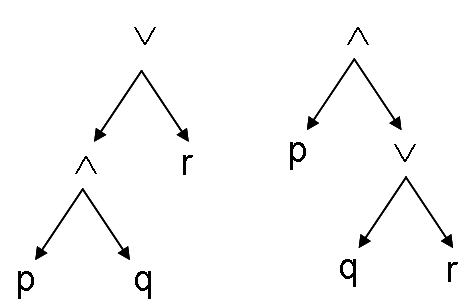
\includegraphics[scale=0.7]{usoparent.png}}
	\end{figure}
	\end{itemize}
\end{frame}

\begin{frame}[t]{Uso de Parênteses} % Título do Frame
	\begin{itemize}
	\item Ordem de Precedência dos conectivos:
	\begin{enumerate}
	\item $\sim$
	\item $\wedge ~ \vee ~ \veebar$
	\item $\rightarrow$
	\item $\leftrightarrow$
	\end{enumerate}

	\item {\sc Exercício:} Monte a representação hierárquica para as expressões abaixo:
	\begin{enumerate}
	\item $p \wedge \sim q$
	\item $p \wedge q \veebar r$
	\item $\sim (p \rightarrow q \vee \sim r)$
	\item $p \wedge q \rightarrow \sim p$
	\item $p \wedge (q \rightarrow \sim p)$
	\item $q \rightarrow p \leftrightarrow r \wedge s \vee \sim t$
	\end{enumerate}
	\end{itemize}
\end{frame}

\begin{frame}[t]{Uso de Parênteses} % Título do Frame
	\begin{itemize}
	\item Ordem de Precedência dos conectivos:
	\begin{enumerate}
	\item $\sim$
	\item $\wedge ~ \vee ~ \veebar$
	\item $\rightarrow$
	\item $\leftrightarrow$
	\item $( \ldots )$
	\end{enumerate}

	\item os símbolos de parênteses ``( )'' são então utilizados como modificadores da ordem de precedência.
	\end{itemize}
\end{frame}

\begin{frame}[t]{Construção de Tabelas-Verdade - Exercícios} % Título do Frame
	\begin{enumerate}
	\item $\sim (p \vee \sim q)$
	\item $\sim (p \rightarrow \sim q)$
	\item $p \wedge q \rightarrow p \vee q$
	\item $\sim p \rightarrow (q \rightarrow p)$
	\item $(p \rightarrow q) \rightarrow p \wedge q$
	\item $q \leftrightarrow \sim q \wedge p$
	\item $(p \leftrightarrow \sim q) \rightarrow \sim p \wedge q$
	\end{enumerate}
\end{frame}

\begin{frame}[t]{Construção de Tabelas-Verdade - Exercícios} % Título do Frame
	Suprimir o maior número de parênteses possível (de forma a não alterar a expressão):
	\begin{enumerate}
	\item $((q \leftrightarrow (r \vee q)) \leftrightarrow (p \wedge (\sim (\sim q))))$
	\item $((p \wedge (\sim (\sim q))) \leftrightarrow (q \leftrightarrow (r \vee q)))$
	\item $(((p \vee q) \rightarrow (\sim r)) \vee ((((\sim q) \wedge r) \wedge q)))$
	\end{enumerate}
\end{frame}

% ============================================================================

%\subsection{Tautologias, Contradições e Contingências}

\begin{frame}[t]{Tautologias, Contradições e Contingências} % Título do Frame
	Tautologia ($\blacksquare$):
	\begin{itemize}
	\item Toda proposição $P_{pqr\ldots}$ que, \underline{independente} dos valores lógicos de suas proposições componentes, resulte sempre em {\bf verdade}.
	\item Exemplo: \begin{center}$\sim (p \wedge \sim p)$ \end{center}

	\vskip 1cm
	
	\begin{center}
	\begin{tabular}{|c|c|c|c|}
	\hline
	$\mathbf{p}$ & $\mathbf{\sim p}$ & $\mathbf{p \wedge \sim p}$ & $\mathbf{\sim(p \wedge\sim p)}$ \\
	\hline
	V & F & F & V \\
	\hline
	F & V & F & V \\
	\hline
	\end{tabular}
	\end{center}

	$$P_p(V, F) = (V, V) = \blacksquare$$
	\end{itemize}
\end{frame}

\begin{frame}[t]{Tautologias, Contradições e Contingências} % Título do Frame
	Outros exemplos:
	\begin{itemize}
	\item $p \vee\sim p$
	\item $p \vee\sim (p \wedge q)$
	\item $p \wedge q \rightarrow (p \leftrightarrow q)$
	\item $p \vee (q \wedge\sim q) \leftrightarrow p$
	\item $p \vee r \rightarrow \sim q \vee r$
	\item $((p \rightarrow q) \rightarrow r) \rightarrow (p \rightarrow (q \rightarrow r))$
	\end{itemize}
\end{frame}

\begin{frame}[t]{Tautologias, Contradições e Contingências} % Título do Frame
	Tautologia ($\blacksquare$):\\
	\begin{center}Princípio da Substituição\end{center}
	\begin{itemize}
	\item Se $P_{pqr\ldots}$ é uma tautologia então $P_{p_0q_0r_0\ldots}$ também será uma tautologia, independente dos valores de $p_0, q_0, r_0, \ldots$ 
	\end{itemize}
\end{frame}

\begin{frame}[t]{Tautologias, Contradições e Contingências} % Título do Frame
	Contradição ($\square$):
	\begin{itemize}
	\item Toda proposição $P_{pqr\ldots}$ que, \underline{independente} dos valores lógicos de suas proposições componentes, resulte sempre em {\bf falsidade}.
	\item Exemplo: \begin{center}$p \wedge \sim p$ \end{center}

	\vskip 1cm

	\begin{center}
	\begin{tabular}{|c|c|c|}
	\hline
	$\mathbf{p}$ & $\mathbf{\sim p}$ & $\mathbf{p \wedge \sim p}$ \\
	\hline
	V & F & F \\
	\hline
	F & V & F \\
	\hline
	\end{tabular}
	\end{center}
	
	$$P_p(V, F) = (F, F) = \square$$
	\end{itemize}
\end{frame}

\begin{frame}[t]{Tautologias, Contradições e Contingências} % Título do Frame
	Outros exemplos:
	\begin{itemize}
	\item $p \leftrightarrow\sim p$
	\item $(p \wedge q) \wedge \sim (p \vee q)$
	\item $\sim p \wedge (p \wedge \sim q)$
	\end{itemize}
\end{frame}

\begin{frame}[t]{Tautologias, Contradições e Contingências} % Título do Frame
	Consistência (ou Contingência -- livro texto):
	\begin{itemize}
	\item Toda proposição $P_{pqr\ldots}$ que não é nem uma tautologia nem uma contradição.
	\item Isto é: pelo menos um $V$ e um $F$ em suas interpretações
	\item Exemplo: \begin{center}$p \rightarrow \sim p$ \end{center}

	\vskip 1cm
	
	\begin{center}
	\begin{tabular}{|c|c|c|}
	\hline
	$\mathbf{p}$ & $\mathbf{\sim p}$ & $\mathbf{p \rightarrow \sim p}$ \\
	\hline
	V & F & F \\
	\hline
	F & V & V \\
	\hline
	\end{tabular}
	\end{center}
	$$P_p(V, F) = (F, V)$$
	\end{itemize}
\end{frame}

\begin{frame}[t]{Tautologias, Contradições e Contingências - Exercícios} % Título do Frame
	Classifique as proposições abaixo como tautológicas, contraditórias (ou insatisfatível ou inconsistente) ou consistentes (ou satisfatível ou contingente):
	\begin{enumerate}
	\item $(p \rightarrow p) \vee (p \rightarrow\sim p)$
	\item $p \rightarrow (p \rightarrow q \wedge\sim q)$
	\item $(p \rightarrow q) \rightarrow (p \vee r \rightarrow q \vee r)$
	\end{enumerate}
\end{frame}
%%%%%%%%%%%%%%%%%%%%%%%%%%%%%%%%%%%%%%%%%%%%%%%%%%%%%%%%%%%%%%%%%
\begin{frame}[t]{Resumindo a nomenclatura dos tipos de fórmulas} % Título do Frame

\begin{block} {}
	\begin{itemize}
	\item Tautológica: sempre verdade ($\blacksquare $)
	\item Contraditórias ou insatisfatíveis ou inconsistentes ($\square$)
	\item Consistentes ou satisfatíveis ou contingentes (pelo menos um $V$ e um $F$ na TV)
	\end{itemize}
\end{block}	
\end{frame}
%%%%%%%%%%%%%%%%%%%%%%%%%%%%%%%%%%%%%%%%%%%%%%%%%%%%%%%%

